\section{ITSA-58-5 Set Partition}
\centerline{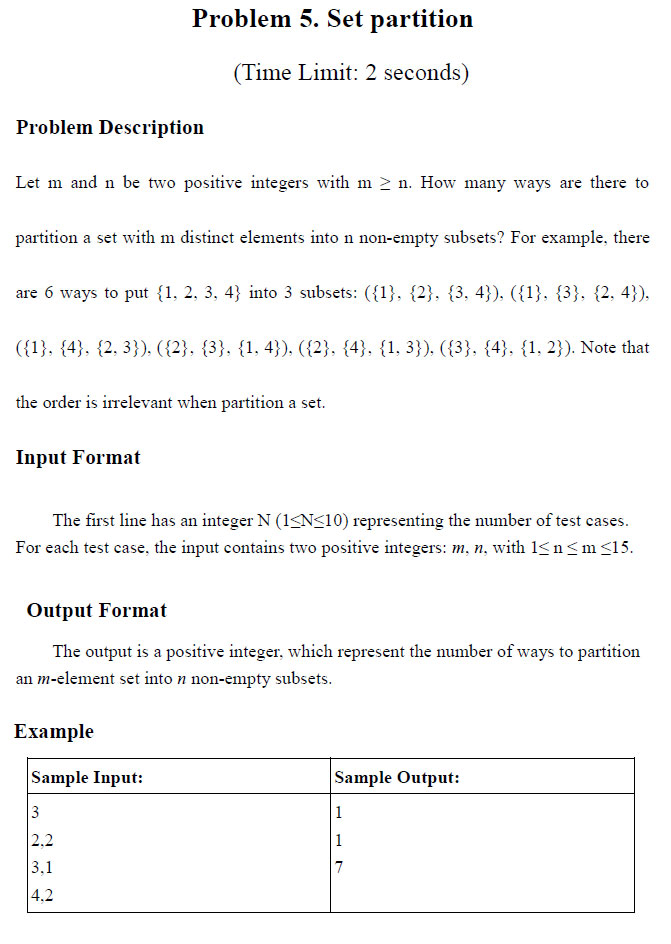
\includegraphics[height=.95\textheight]{../solutions/fig/58ITSA5}}

\subsection{解題思惟}
\begin{enumerate}
	\item 這一題要直接找到公式計算的話,看起來挺困難的。不過使用遞迴的角度去思考,會發現並沒有那麼難。
	\item 假設m個數字$1,2,\cdots,m$分成n堆的所有可能數目是f(m,n)。現在我們先把1拿出來單獨考慮,這時只有兩種情況,一種是1自己一堆,另一種是1跟其他數字一堆。
	\item 如果1自己一堆的話,那麼剩下的堆數是n-1,而且只有m-1個數,所以總共的可能數目會是f(m-1, n-1)。
	\item 如果1跟別人一堆的話,那麼先不考慮1,就是m-1個數有n堆,所以可能的數目會是f(m-1, n)。接著考慮1會放在哪一堆呢?放哪一堆都有可能,也就是有n種放法。這樣的話,總共的可能數目變成$n\times f(m-1, n)$。這裡面會不會有重複的情況發生呢?如果有兩種分法是相等的,那麼1的那堆數字要相同,其他的n-1堆不管順序的也要相同,那把1拿掉,這兩種分法等於也是相同的,但我們所用的f(m-1, n)的定義,就是不同的分法,所以就違反我們的假設了,因此不會有重複的情況發生。
	\item 根據以上的分析,我們已經找到遞迴的規則。接下來要找終止條件,這個比較容易,就是當n=1的時候,表示只有一堆,也只有一種分法;當n=m的時候,表示分成m堆,等於每個數各自一堆,也只有一種分法。
\end{enumerate}

\subsection{程式碼}
\begin{cppcode}
#include <iostream>

using namespace std;

int f(int m, int n);

int main()
{
	int kase, m, n;
	cin >> kase;
	while (kase--) {
		char c;
		cin >> m >> c >> n;
		cout << f(m, n) << endl;
	}
	return 0;
}

int f(int m, int n)
{
	if (n==1 || n==m) return 1;
	return f(m-1, n-1) + n*f(m-1, n);
}
\end{cppcode}